\subsection{Test Configuration}

Our benchmark was tested on a 72-core (4 sockets with 18 cores each capable of running 2 hardware threads, totaling 144 hardware threads) Intel Xeon machine clocked at 2.50 GHz with 512 GB of RAM and 4 memory banks. The machine is running Ubuntu 14.04 with kernel verion 3.13.0-141. The with DEF code was compiled with DEF version 0.16.1a and the C code was compiled with Clang 6.0, and all code was compiled with -03 level of optimisation.

During the benchmark threads were pinned programmatically to inidvidual cores initially avoiding HyperThreading and later exhausting all inidivual exection units on a single CPU with the use of HyperThreading, before migrating to another CPU socket. JEMalloc\cite{JEMalloc} was used in all tests, as it had been in the Forkscan paper.\cite{Forkscan} The \texttt{numactl} Linux program was used to control which memory bank allocation was allowed to take place. The memory banks closest to the running CPUs were selected as they became active.

The microbenchmark measures the number of operations carried out over a specified amount of time rather than the time taken to exectute a specified number of iterations. The rationale for this is threads finish their iterations before other threads. The remaining threads complete their iterations with less contention in the system, skewing the overall benchmark. Our benchmark reports the number of operations per second. The primary comparison is between the leaky C and the forkscan enabled DEF implementations. Each benchmark is run for a total of 20 seconds each, with each configuration being sampled 5 times. The average of the runs is plotted with error bars show the maximum variation in each run.

\subsection{Benchmark Results}

\begin{figure}[htbp!]
  \centering
  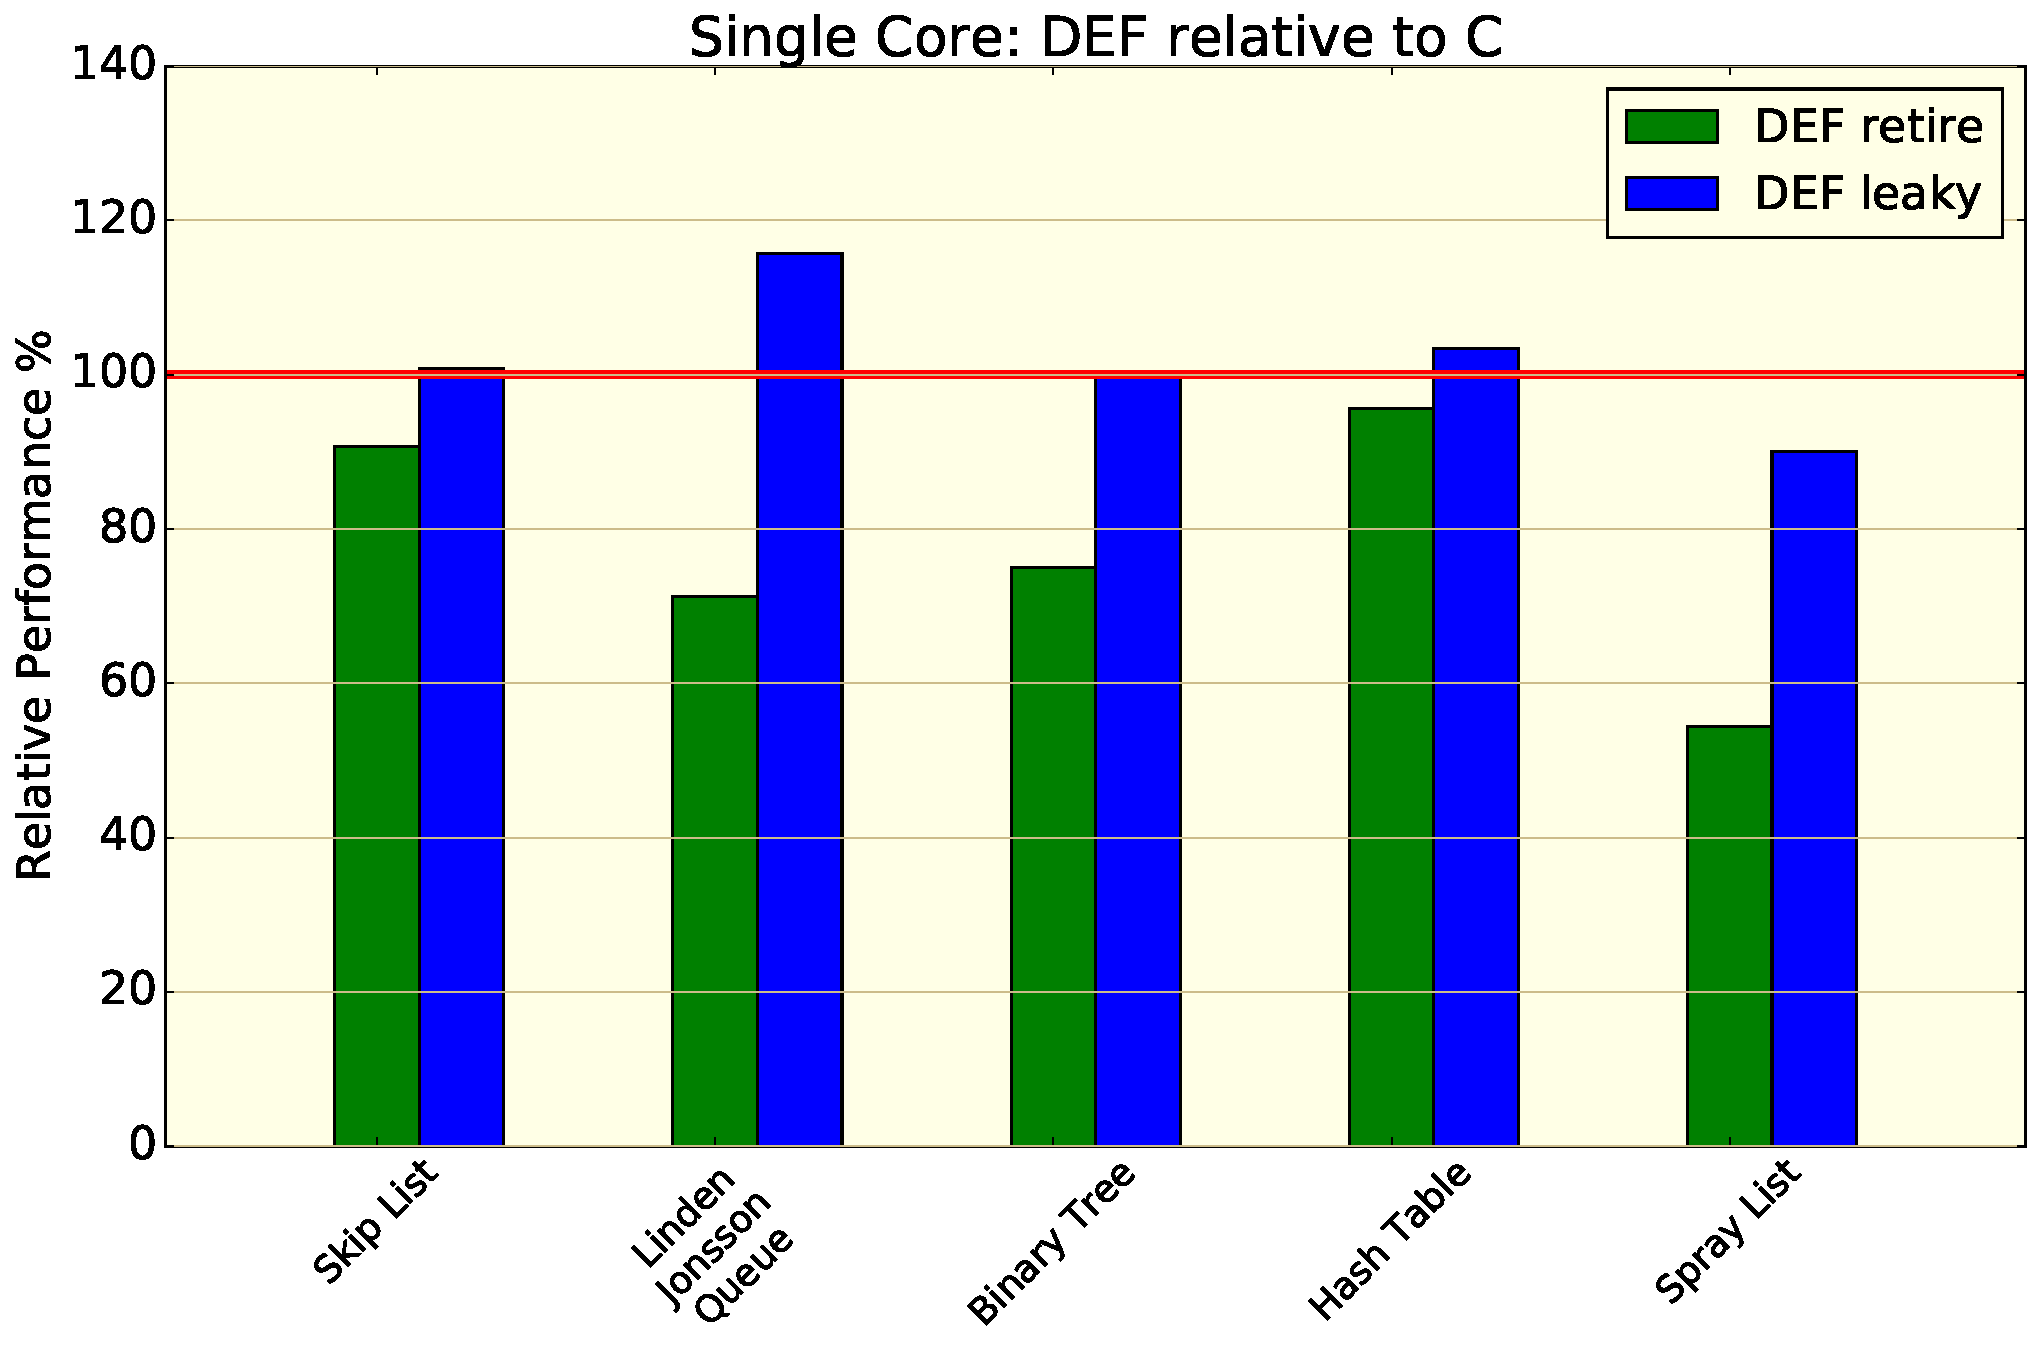
\includegraphics[scale=0.25]{gfx/RelativePerf.pdf}
  \caption{Relative performance of DEF to C on a single thread.  100\% is equivalent, and higher is better.}
  \label{fig:relativeperf}
\end{figure}

Figure \ref{fig:relativeperf} shows, for all benchmarks, single-threaded performance.  The set data structures are configured with 10\% updates, and the priority queue, naturally, are 100\% updates.  For an apples-to-apples comparison with C, a non-retiring version of the DEF code is presented.  This is a meaningful test because one expects a serial C data structure to perform better when \texttt{free} is never called than when it is, and it's no different for a concurrent data structure.  As designed, DEF is close to the machine and performs comparably in this case.  We attribute any performance distinctions to slight differences in code generation.

Minor degradation in performance is observed when memory is retired. (results?)

\begin{figure*}[tbp]
  \centering
  \raisebox{-0.5\height}{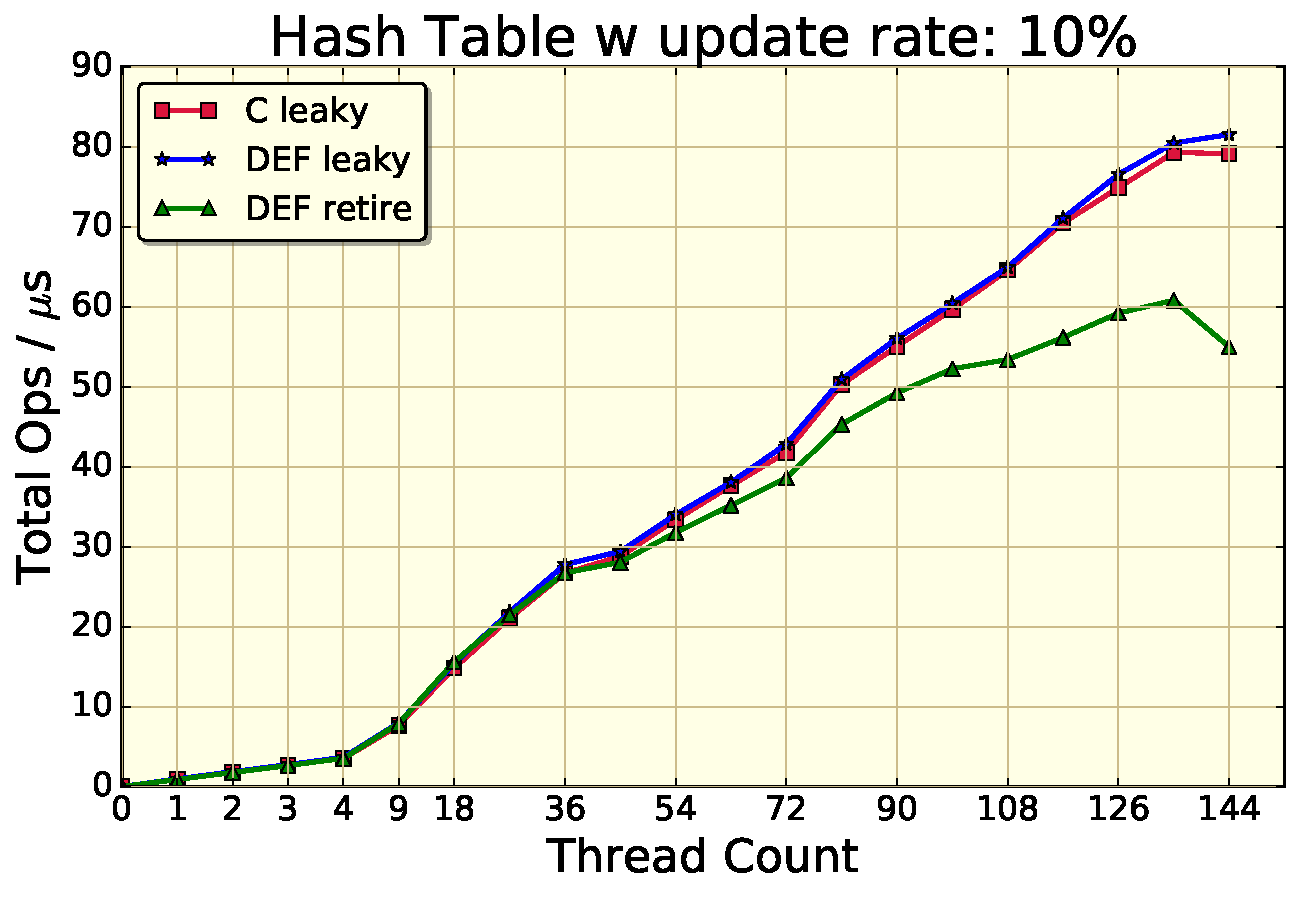
\includegraphics[scale=0.25]{gfx/HashTableLight.pdf}}
  \raisebox{-0.5\height}{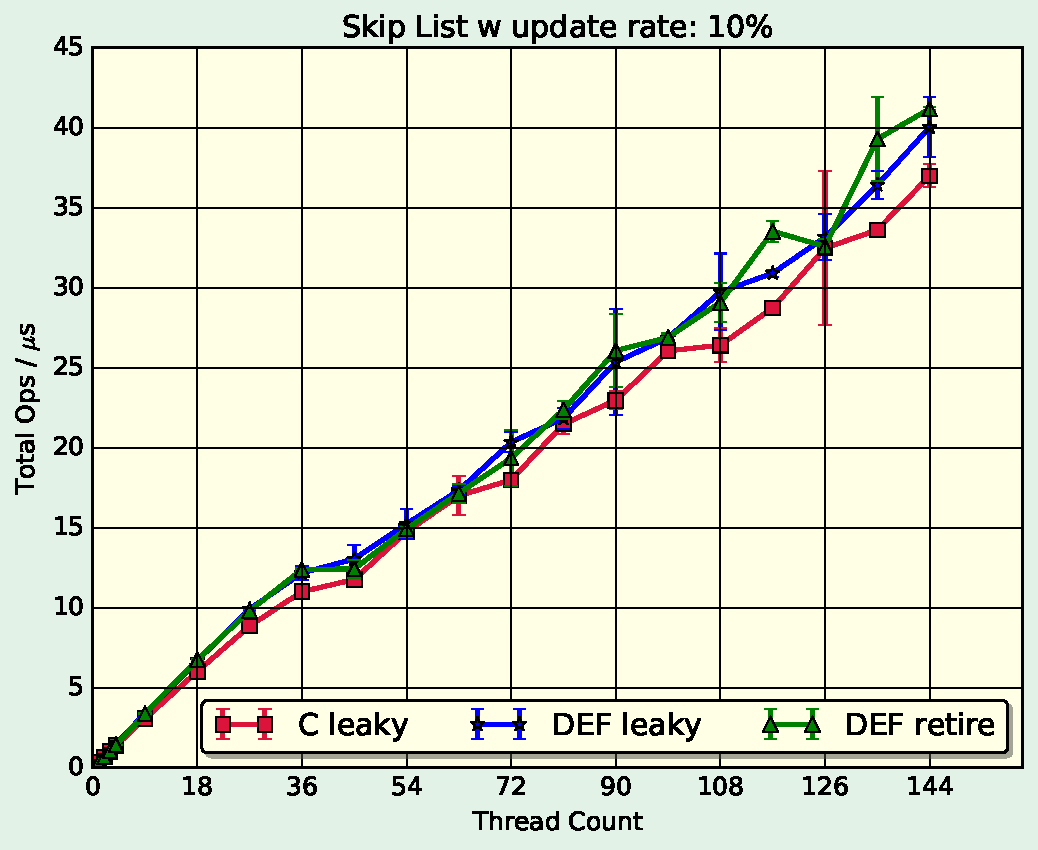
\includegraphics[scale=0.25]{gfx/SkipListLight.pdf}}
  \raisebox{-0.5\height}{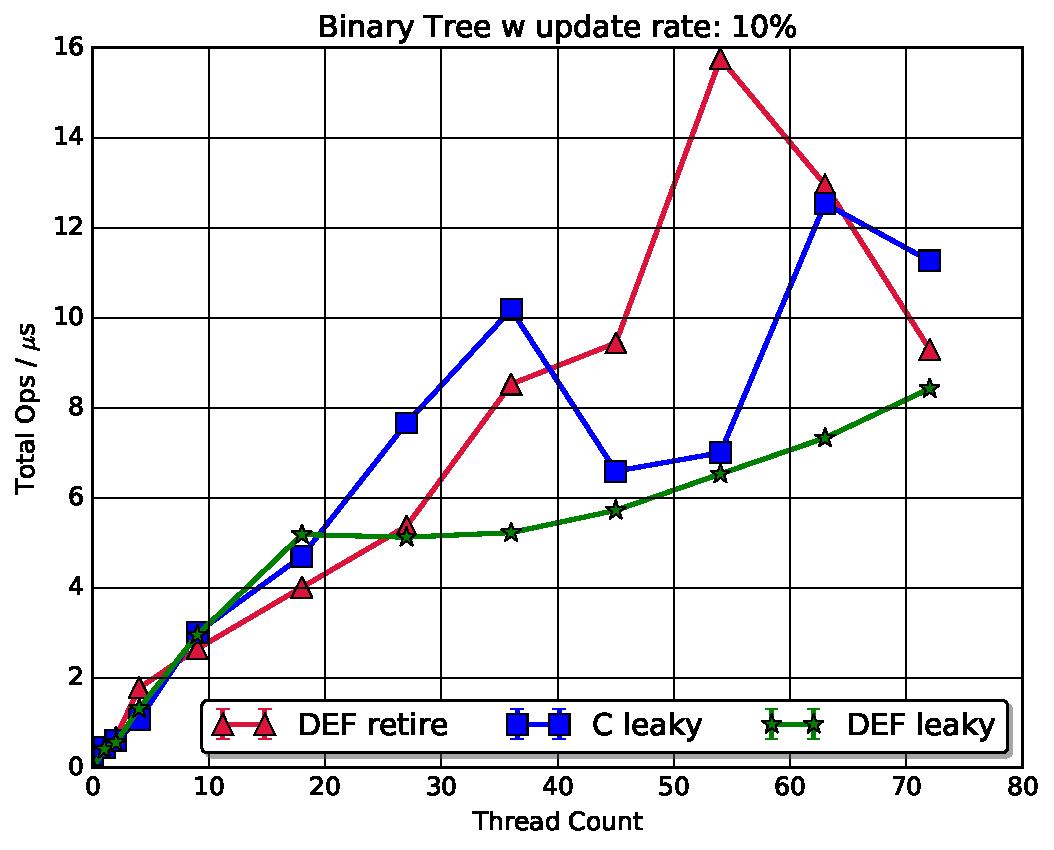
\includegraphics[scale=0.25]{gfx/BinaryTreeLight.pdf}}
  \raisebox{-0.5\height}{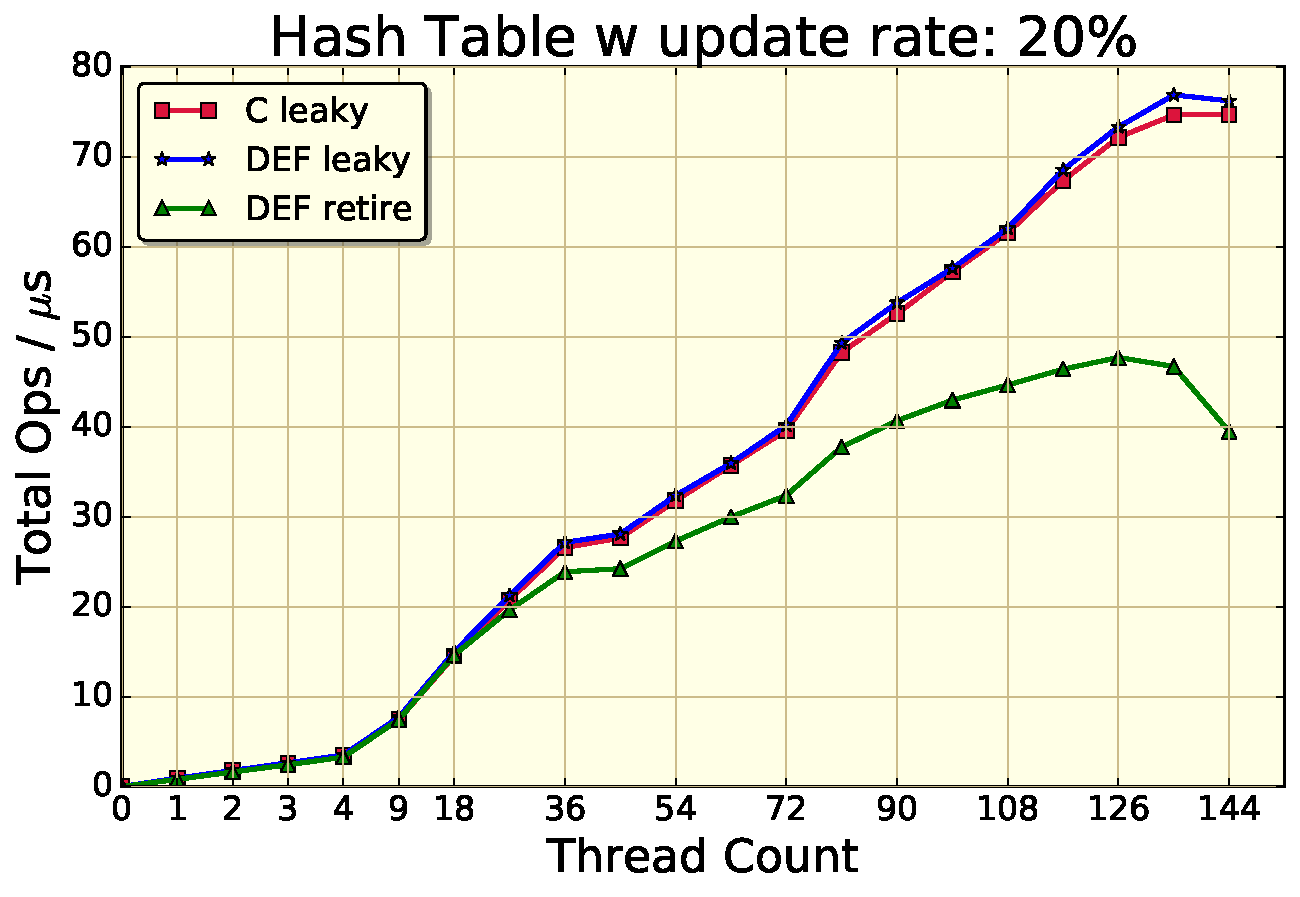
\includegraphics[scale=0.25]{gfx/HashTableMedium.pdf}}
  \raisebox{-0.5\height}{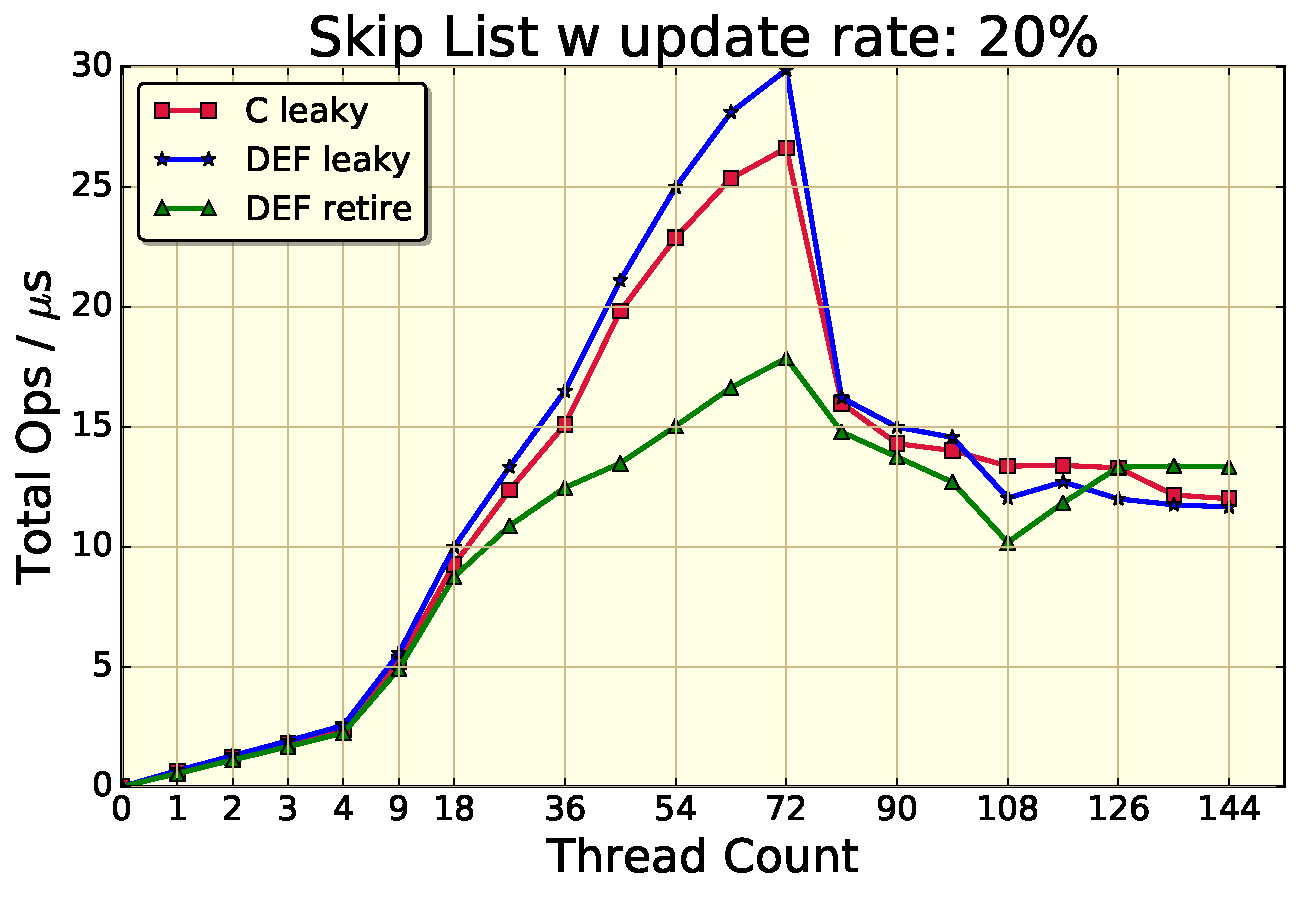
\includegraphics[scale=0.25]{gfx/SkipListMedium.pdf}}
  \raisebox{-0.5\height}{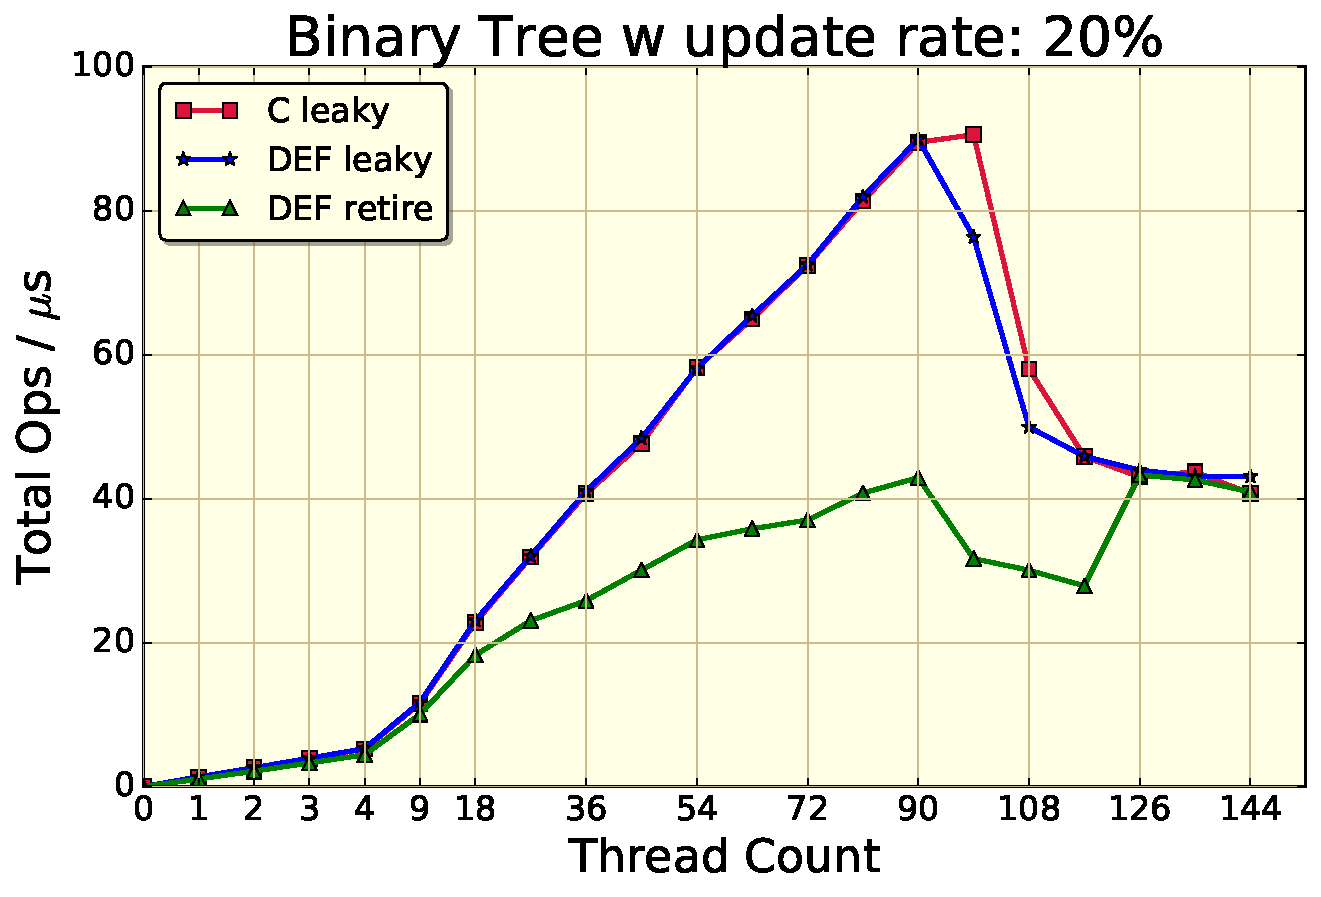
\includegraphics[scale=0.25]{gfx/BinaryTreeMedium.pdf}}
  \caption{Scalability graphs for the set data structures with 10\% (top row) and 20\% (bottom row) updates.}
  \label{fig:setdatastructures}
\end{figure*}

Scalability results for the set data structures with 10\% and 20\% updates are presented in figure \ref{fig:setdatastructures}.  20\% updates, on a set data structure, represents an extremely heavy workload.  10\% represents something more typical.  As above, the three configurations were tested: Leaky-DEF, DEF, and C (also leaky).

% Hashtable: node = 24
% Tree: node = 24
% Skip List: node = 172 (height 20)
% Shavit/Lotan: node = 180 (height 20)
% SprayList: node = 180 (height 20)

C and Leaky-DEF both scale similarly for all three structures.  The hash table scales linearly, performing only a few operations per microsecond worse on 144 threads at 20\% than at 10\%.  In the retiring version of the code, Forkscan is able to keep pace until the application saturates the first socket at 36 threads.  The decline at the high end is due to the fact that Forkscan creates a pool of child processes to perform its scan, up to 16, but since the application threads are pinned, the Forkscan threads get shifted around.

The skip list saturates the memory bandwidth with its enormous fixed-height nodes.  The peaks are merely shifted left in the 20\% executions versus 10\%, and don't rise as high (35 vs. 60 ops/$\mu$s).  Leaky DEF scales more quickly and, consequently, falls off sooner than the C version.  This is related to the aforementioned difference in code generation.  Nodes average two pointers instead of one, as in the hash table, making root finding slower when memory is reclaimed.  But its decline has the same cause as the leaky implementations: it hits the memory bandwidth at the same time.

The binary tree tests the limits of the memory reclamation implementation, which scales with the leaky versions, but has a more gradual slope.  At 10\% it declines at the end, just as the hash table did, and for the same reason.  The binary tree, exceeding the performance of this hash table, involves more writing per update.  At 20\% updates, the leaky versions reach the memory bandwidth limits before they've run out of physical threads.

\begin{figure*}[tbp]
  \centering
  \raisebox{-0.5\height}{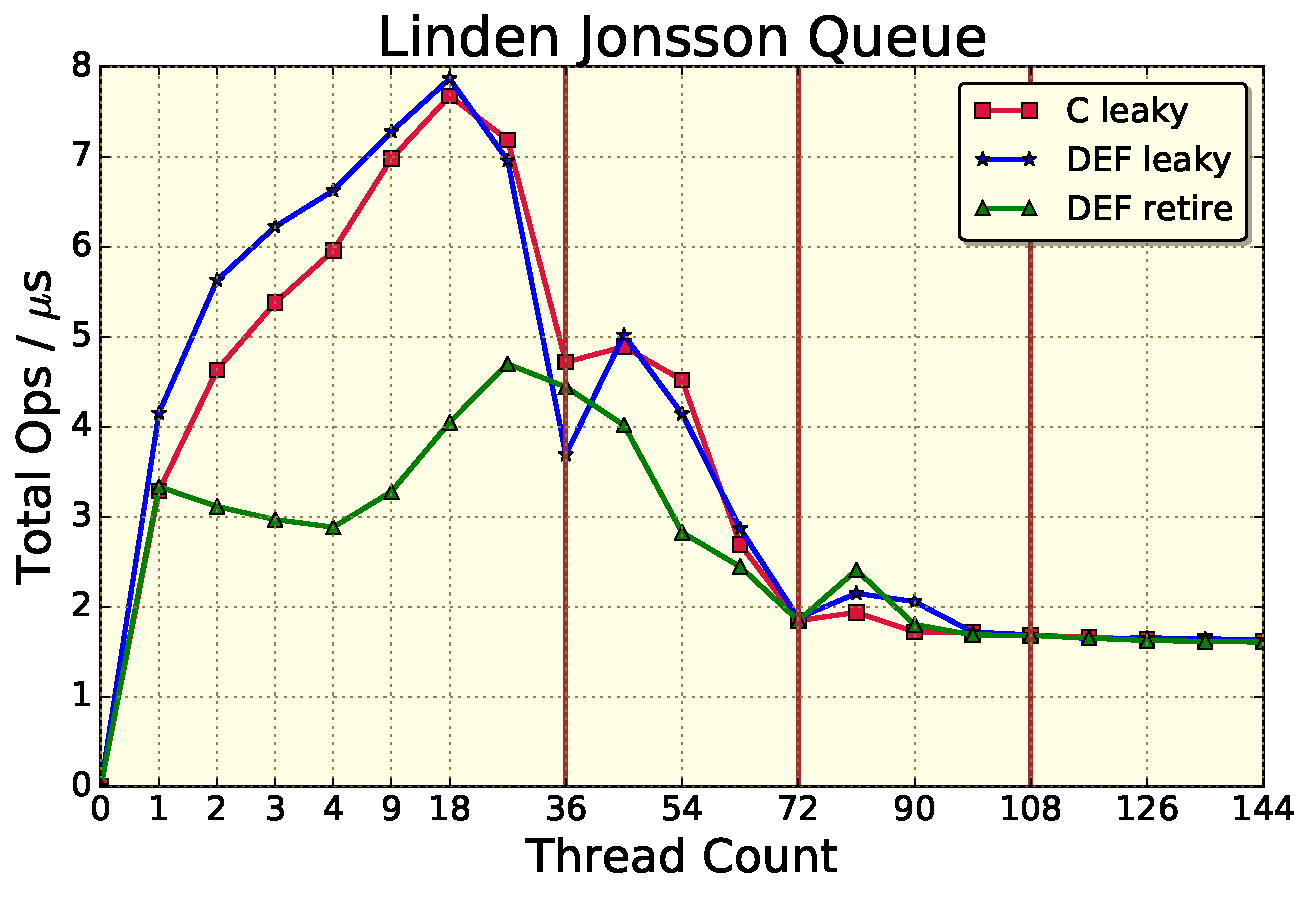
\includegraphics[scale=0.25]{gfx/LindenJonssonQueue.pdf}}
  \raisebox{-0.5\height}{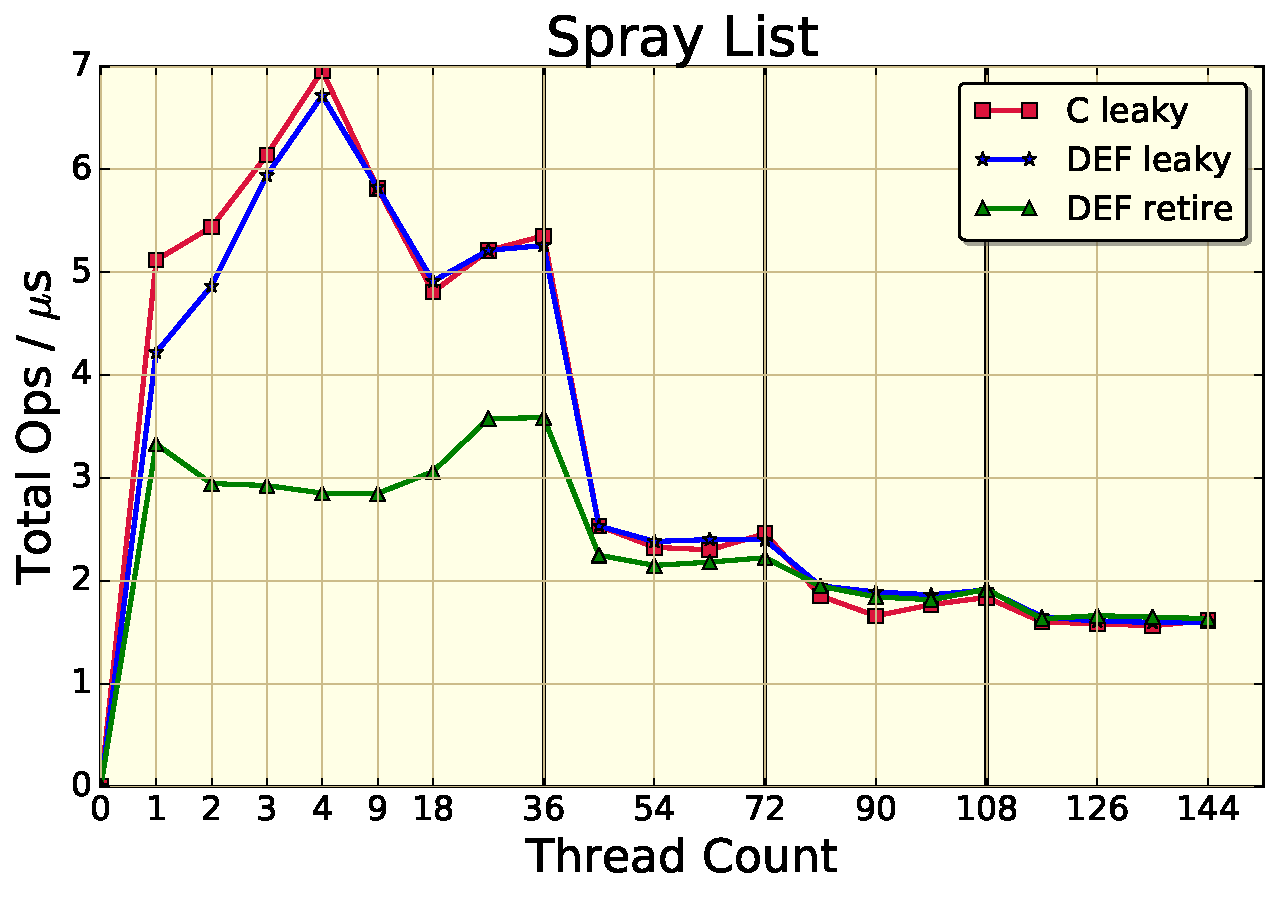
\includegraphics[scale=0.25]{gfx/SprayList.pdf}}
  \caption{Scalability graphs for the priority queues. The priority queues standard workload is 100\% updates.}
  \label{fig:priorityqueues}
\end{figure*}

Lastly, in figure \ref{fig:priorityqueues}, we tested the SprayList priority queue.  The leaky implementations took a performance hit crossing the NUMA node boundary at 36 cores and never recovered.  One of the difficulties with a skip list-based priority queue is that many threads have a few early nodes in common in their caches.  As thread-counts increase, so do the number of invalidations, leading to the shape of the graph.  This is a worst-case data structure for Forkscan because priority queues are entirely updates, and the nodes are big (180 bytes, in this implementation).  However, again, the retiring DEF implementation has the same shape as the leaky ones.  It scales while they scale, and it's ultimately defeated by the same hurdle.

In all of these structures, reclaiming memory scales up to the physical limits of the hardware, albeit with a gentler slope.  We attribute this to the on-demand aspect of memory tracking, versus at-allocation tracking; the memory that gets retired can mostly be deallocated.  Very little has to be recursively searched.

